\chapter{$K^- d \rightarrow K^0 n n$ events}
\begin{figure}[htbp]
  \centering
  \begin{tabular}{cc}
    \begin{minipage}{0.5\hsize}
      \includegraphics[width=6cm]{../pic/Run78/QE/mmN_mom_woFit.eps}
    \end{minipage}
    \begin{minipage}{0.5\hsize}
      \includegraphics[width=6cm]{../pic/Run78/QE/IM_nK0_woFit.eps}
    \end{minipage}
  \end{tabular}
  \caption{
    Left figure indicates missing neutron momentum distribution in $d(K^-, n K^0)"n"$ events.
    Right figure indicates invariant mass of $n K^0$ in same event sample.
  }
  \label{fig:K0_mom_IM_woFit}
\end{figure}
\begin{figure}[htbp]
  \centering
  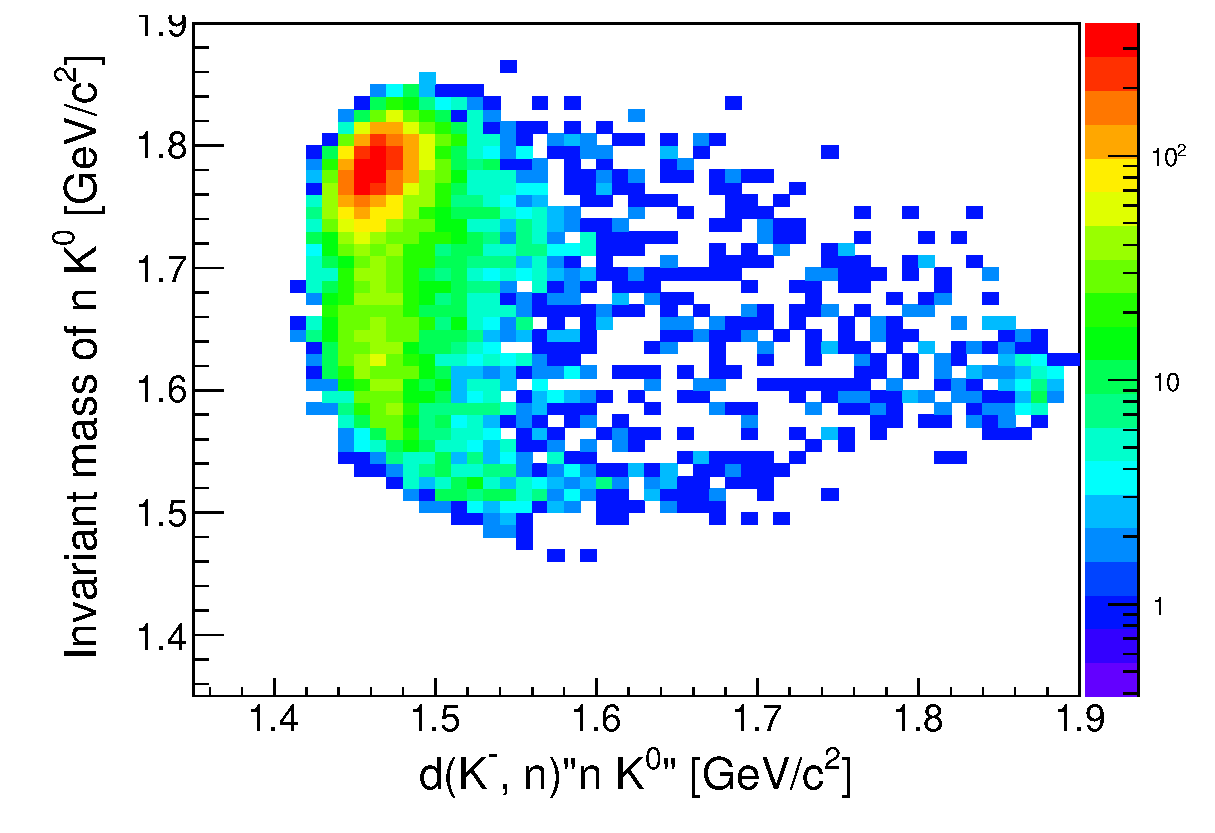
\includegraphics[width=8cm]{../pic/Dron/KN_MM_nK0_IM.eps}
  \caption{
    This figure represents scatter plot of the $d(K^-, n)"n K^0"$ and invariant mass of the $n K^0$ which are detected particles.
  }
  \label{fig:KN_MM_IM_nK0}
\end{figure}
In the $d(K^-, n)"n K^0"$ reaction, the missing neutron momentum disribution should be corresponding to fermi motion distribution.
Invariant mass distribution of $n_{detected} K^0$ should also be distributed just below the kinematical threshold which is about $1.8GeV/c^2$ with $1GeV/c^2$ $K^-$ beam.
On the other hand, the missing neutron momentum distribution was observed high momentum component
and the invariant mass of $n_{detected} K^0$ was observed widly distributed component in the data as Fig\ref{fig:K0_mom_IM_woFit}.
Such widly distribution is not observed in the $d(K^-, n)"n K^0"$ distribution as Fig\ref{fig:KN_MM_IM_nK0}.

\begin{figure}[htbp]
  \begin{tabular}{cc}
    \begin{minipage}{0.5\hsize}
      \begin{tikzpicture}
        \begin{feynhand}
          \vertex[particle] (Km)     at (-2.0,  1.5) {$K^-$};
          \vertex[particle] (d)      at (-2.0, -1.0) {$d$};
          \vertex[particle] (n_det)  at ( 2.0,  1.5) {$n_{detected}$};
          \vertex[particle] (K0)     at ( 2.0,  0.0) {$K^0$};
          \vertex[particle] (n_miss) at ( 2.0, -1.0) {$n_{missing}$};
          \vertex (w1) at (0, 0.5);
          \propag [fermion] (Km) to (w1);
          \propag [fermion] (d)  to (w1);
          \propag [fermion] (w1) to (n_det);
          \propag [fermion] (w1) to (K0);
          \propag [fermion] (d)  to (n_miss);
        \end{feynhand}
      \end{tikzpicture}
    \end{minipage}
    \begin{minipage}{0.5\hsize}
      \begin{tikzpicture}
        \begin{feynhand}
          \vertex[particle] (Km)     at (-2.0,  1.5) {$K^-$};
          \vertex[particle] (d)      at (-2.0, -0.3) {$d$};
          \vertex[particle] (n_det)  at ( 2.0,  1.5) {$n_{detected}$};
          \vertex[particle] (K0)     at ( 2.0,  0.0) {$K^0$};
          \vertex[particle] (n_miss) at ( 2.0, -1.0) {$n_{missing}$};

          \vertex[particle] (Kbar) at ( 0.3, 0.1) {$\bar{K}$};
          \vertex (w1) at (0,  0.5 );
          \vertex (w2) at (0, -0.3);
          \propag [fermion] (Km) to (w1);
          \propag [fermion] (d)  to (w1);
          \propag [fermion] (d)  to (w2);
          \propag [fermion] (w1) to (n_det);
          \propag [fermion] (w1) to (w2);
          \propag [fermion] (w2) to (K0);
          \propag [fermion] (w2)  to (n_miss);
        \end{feynhand}
      \end{tikzpicture}
    \end{minipage}
  \end{tabular}
  \caption{
  }
  \label{fig:KD_K0NN_fyen}
\end{figure}

Fig\ref{fig:KD_K0NN_fyen} indicates feynmman daiagram of 1-step reaction and 2-step reaction of $K^- d\rightarrow K^0 n n$ final state.
$d(K^-, n)"n K^0"$ spectrum strongly reflects to 1-step $\bar{K}N$ scattering,
on the other hand invariant mass of $n_{detected} K^0$ strongly reflects to interaction between recoiled $\bar{K}$ and residual nucleon.
We simulated this reaction using following simply assamption.
The 1-step reaction was simulated quasi-elastic scattering of $K^- p\rightarrow K^0 n$ reaction and recoild $K^0$ rescattered with residual nucleon isotropically.
In left figure of Fig\ref{fig:K0_mom_IM_woFit}, a bump structure around $\Lambda(1520)$ is seen.
So, We also simulated $K^- n \rightarrow n_{forward} \Lambda(1520)$ reaction.\\
We perfom fitting for invariant mass spectra to estimate ratio of 2-step like reaction.
In this fitting, strength of $\pi^{\mp}\Sigma^{\pm}$ was fixed and quasi-elastic (1-step) reaction, quasi-elastic with rescattering (2-step) reaction and $\Lambda(1520)$ production were free parameters.
Fitting result indicats left figure of Fig\ref{fig:fit_IM_nK0}.
The momentum distribution of $n_{missing}$ and $d(K^-, n)"n K^0"$ were also shown in same figures.\\
According to this fitting, we obtained that the rations of 1-step, 2-step and $\Lambda(1520)$ production is 80\%, 12\% and 8\% in $K^- d \rightarrow K^0 n n$ final state.

\begin{figure}[htbp]
  \begin{tabular}{ccc}
    \begin{minipage}{0.33\hsize}
      \includegraphics[width=4.5cm]{../pic/Run78/K0_ts/fit_KN_IM_npipi_K0_ts_L1520.eps}
    \end{minipage}
    \begin{minipage}{0.33\hsize}
      \includegraphics[width=4.5cm]{../pic/Run78/K0_ts/fit_mmN_momK0_ts_L1520.eps}
    \end{minipage}
    \begin{minipage}{0.33\hsize}
      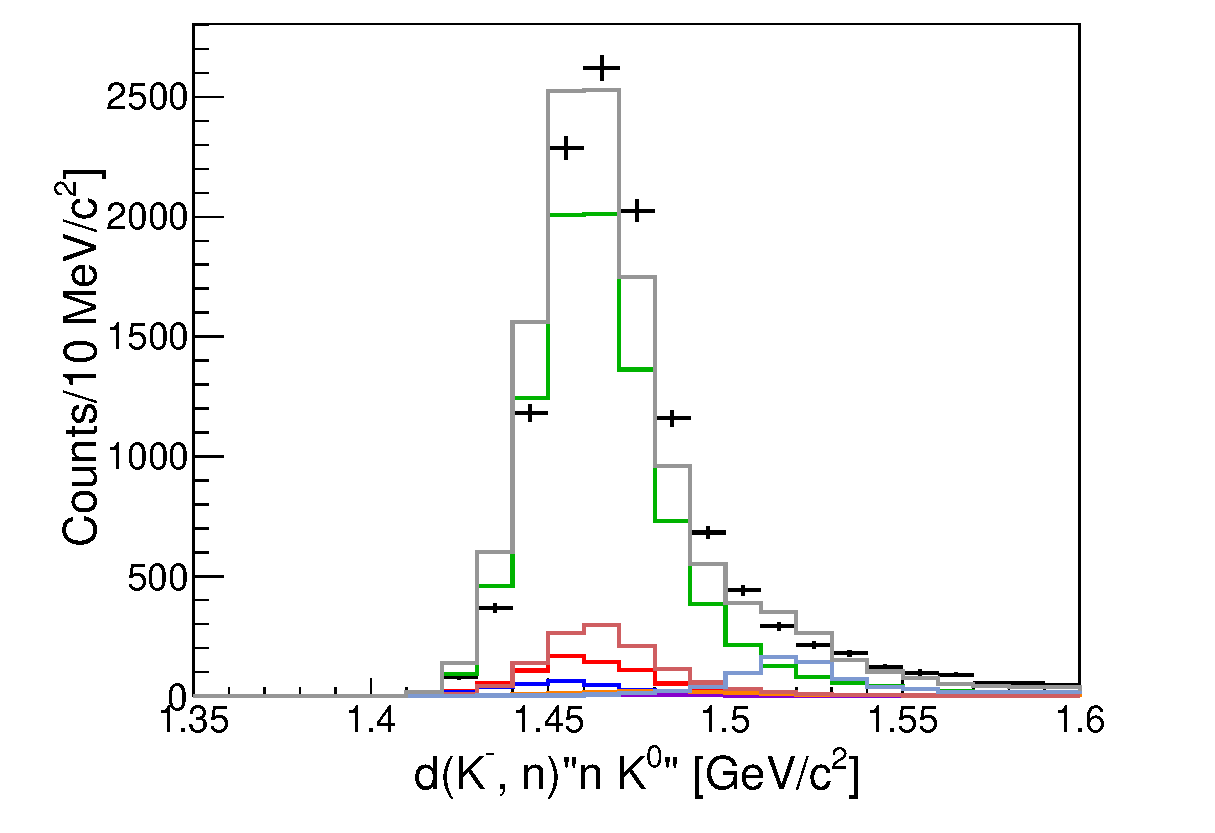
\includegraphics[width=4.5cm]{../pic/Run78/K0_ts/fit_KN_MM_K0_ts_L1520_after.eps}
    \end{minipage}
  \end{tabular}
  \caption{
  }
  \label{fig:fit_IM_nK0}
\end{figure}

